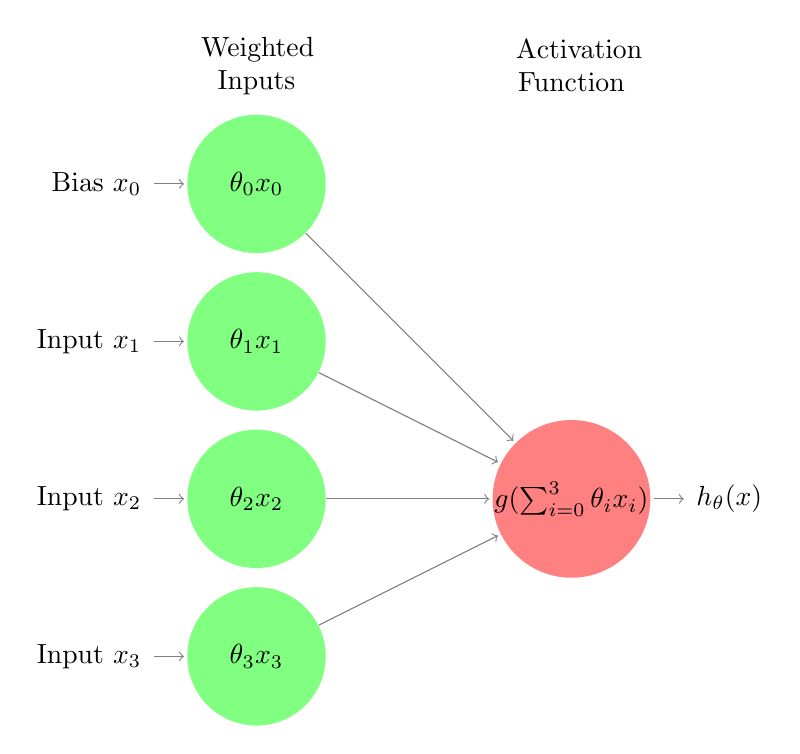
\begin{tikzpicture}[shorten >=1pt,->,draw=black!50, node distance=2.5cm]
    \tikzstyle{every pin edge}=[<-,shorten <=1pt]
    \tikzstyle{neuron}=[circle,fill=black!25,minimum size=50pt,inner sep=0pt]
    \tikzstyle{input neuron}=[neuron, fill=green!50];
    \tikzstyle{output neuron}=[neuron, fill=red!50];
    \tikzstyle{hidden neuron}=[neuron, fill=blue!50];
    \tikzstyle{annot} = [text width=4em, text centered]

    % Draw the input layer nodes
 %   \foreach \name / \y in {0,...,3}
    % This is the same as writing \foreach \name / \y in {1/1,2/2,3/3,4/4}
        \node[input neuron, pin=left:Bias $x_0$] (I-0) at (0,-0) {$\theta_0 x_0$};
	\foreach \name / \y in {1,...,3}
    % This is the same as writing \foreach \name / \y in {1/1,2/2,3/3,4/4}
        \node[input neuron, pin=left:Input $x_{\y}$] (I-\name) at (0,-2*\y) {$\theta_{\y}x_\y$};
    % Draw the hidden layer nodes
    %\foreach \name / \y in {1,...,5}
     %   \path[yshift=0.5cm]
      %      node[hidden neuron] (H-\name) at (\layersep,-\y cm) {};

    % Draw the output layer node
    \node[output neuron,pin={[pin edge={->}]right:$h_{\bm{\theta}}(x)$}, right of=I-2, node distance=4cm] (O) {$g(\sum^3_{i=0}\theta_ix_i)$};

    % Connect every node in the input layer with every node in the
    % hidden layer.
   % \foreach \source in {1,...,4}
    %    \foreach \dest in {1,...,5}
     %       \path (I-\source) edge (H-\dest);

    % Connect every node in the hidden layer with the output layer
    \foreach \source in {0,...,3}
        \path (I-\source) edge (O);

    % Annotate the layers
%    \node[annot,above of=H-1, node distance=1cm] (hl) {Hidden layer};
    \node[annot,above of=I-0, node distance=1.5cm](il) {Weighted Inputs};
    \node[annot,right of=il, node distance=4cm] {Activation Function};
\end{tikzpicture}